\documentclass[main]{subfiles}

\begin{document}
% Chapter Template
\setcounter{chapter}{1}

% Evolutionary Optimization
% Basic components
%  Universe, Planets and Environments
%   Planet Physics
%  Epochs
%   Fitness functions
%  Populations
%  Creatures
%   Genotypes
%   Phenotypes
%    Constrained Rigid body model
%    Featherstone Multi-rigidbody model
%  Model organisms
% Reaper
%  Crossover
%  Mutations
% Evaluation Step
% Variation Step
\chapter{Evolutionary Optimization} % Main chapter title

\label{Chapter\thechapter} % Change X to a consecutive number; for referencing this chapter elsewhere, use \ref{ChapterX}

\lhead{Chapter \thechapter. \emph{Evolutionary Optimization}} % Change X to a consecutive number; this is for the header on each page - perhaps a shortened title

The following chapter describes the Evolutionary optimization algorithm as it is implemented in the Minemonics simulator. The Minemonics simulator is a project that was developed from scratch for this Thesis, mainly because most other simulators for evolving virtual creatures are unpublished by the research group, outdated or implement a different type of simulation than is needed for the model of this thesis.

\section{Basic components}

First, the basic components of the simulator are listed and its features are described. We describe the component tree in a top-down manner and reveal the subcomponents one-by-one. 

%-----------------------------------
%	SUBSECTION 1
%-----------------------------------
\subsection{Universe, Planets and Environments}

The simulator models its own universe. A universe contains a set of different planets, each being a certain setting of evolutionary run. A certain planet consists of an environment, a evolution type, a number of epochs and a number of populations. 

The environment simulates a flat plane or a hill environment. It approximates the appropriate newtonian mechanical physics for the environment and the creatures that are evaluated within it. For the experiments in this thesis, mainly the plane environment was used.

The evolution type defines how many creatures of the planet are evaluated at the same time and how creatures are culled, variated and sown. In the bounds of this thesis, only single creature evaluation was performed. 

\subsubsection{Planet physics}

Each environment defines the planet's physics simulation. The simulator uses the Bullet Physics engine\cite{bulletphysics} to run the physical simulation of the creatures. Bullet Physics is a numerical classial mechanics simulation engine, featuring rigid body as well as softbody physics. Bodies can be constrained using various types of constraints with constraint limits and motors. The constraints are numerically solved using one of the many types of solvers with different convergence speeds and accuracy of result. The most accurate results were achieved using the Featherstone Multibody solver. To date it only supports single degree of freedom joints, however this does not affect the evolutionary optimization much. A three degrees of freedom joint can easily be approximated by three one degree of freedom joints.

\subsection{Epochs}

An epoch of a certain planet models the changes of environmental factors, which induce modification of the fitness landscape on the planet. What is considered good in one epoch might not be good in another. The change of the fitness landscape usually leads to avalanches of extinction[?]. A certain epoch in the simulation consists of a set of juries(fitness functions) and a transition condition, which, when met, ends the epoch and starts the next epoch.

\subsubsection{Juries}

Juries or fitness functions are part of an epoch in which they are relevant. A jury collects data on a certain performance during the evaluation of a creature and finally has to rate the performance of an individual. Commonly used juries of the simulator are the distance travelled during the evaluation time or the average height of all limbs during the evaluation. A jury additionally has a weight, which indicates the weight in the total performance of the creature, and a sorting direction, which indicates whether a higher rating is considered better or worse than a lower rating. Multiple types of juries are combined in a competitive manner among the creatures of a population. This procedure will be described in the section \ref{subsubsection:Culling} Culling of the Reaper component.

\subsection{Populations}

A population of creatures on the simulator lives on a certain planet. Depending on the evolution settings of the planet, one creature, multiple creatures of one population, multiple creatures of multiple populations or multiple whole populations are evaluated within one evaluation time. When a population is initialized, it it has a certain initial number of individuals. These can be completely randomly generated creatures or model organisms, the being common primitives for testing. During the evaluation of a population, the number of individuals falls generally below the original population size, because several individuals are culled during the evaluation. This happens when creatures surpass boundaries of physical realism (generally high forces that lead to very fast limb velocity, leading to imaginary forces that lift creatures off the ground and make them fly) which causes the simulation to cull them early and set their fitness to the lowest value. 

\subsection{Creatures}

A creature or individual is part of a population and is subject to evaluation. The creature is based on two main components. Its genotype and its phenotype. The genotype is the compact blueprint of the creature. Developed from it is the phenotype, which is the explicit form of the creature representing the body of the creature in the Physics engine and the controller in its fully wired form. Furthermore we define to important measures for creatures which are its total body volume and its size. The total body volume is just the volume of all limbs summed up. The size of a creature is measured as being the third root of the total volume, denoting the edge length of the total volume cube. The size measure is most important because it is used to scale the fitness functions involving distances. Thereby it is possible to make a distance travelled independent of the creature size, meaning that a larger creature gets the same fitness as a smaller creature for travelling a larger distance, if the ratio between creature size and respective travelled distance are the same for both creatures.

\subsubsection{Genome}

In the traditional approach on genomes, a fixed length string of bits is used to encode higher order data types such as integers or doubles or into data structures such as trees or matrices. However, many state-of-the-art genomes deviate from this original representation by directly using higher order representations and thereby avoiding the usually hard to solve representation problem ('What representation should be chosen so that every change in the bit string leads to a new valid representation?'). This more modern approach was also chosen in the Minemonics simulator.\\

The genomic model is one of the base models of the simulator. It encodes both morphology and the controller of the creature. Inspired by biological DNA, the genome of the simulator uses an indirect encoding. An indirect encoding, different from a direct encoding, does not encode every element of the phenotype explicitly, but uses element classes and branches between them to encode their relations. 

\begin{figure}[H]
\center
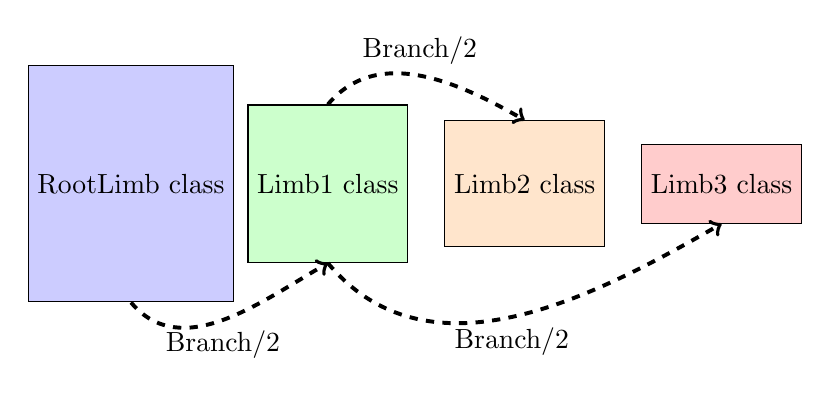
\begin{tikzpicture}
   \foreach \c/\i/\t [count=\n] in  
        {blue!20/RootLimb class/1.5,green!20/Limb1 class/1,orange!20/Limb2 class/0.8,red!20/Limb3 class/0.5} 
           \node[draw,fill=\c,minimum height=\t * 2cm,minimum width = \t * 1cm,xshift=\n* 2.5cm](N\n){\i} ;
\draw[dashed,->,line width=0.5mm] (N1.south) to [out=-50,in=-150] node[below] {Branch/2} (N2.south);
\draw[dashed,->,line width=0.5mm] (N2.north) to [out=50,in=150] node[above] {Branch/2} (N3.north);
\draw[dashed,->,line width=0.5mm] (N2.south) to [out=-50,in=-150] node[below] {Branch/2} (N4.south);

\end{tikzpicture}
\caption{The general structure of the genotype (strongly simplified). The number at the branch denotes the number of child limbs of the following type are attached to the respective parent limb.}
\label{figure:genotype}
\end{figure}


\begin{figure}[!h]
\centering
\missingfigure[figwidth=1\textwidth]{Figure showing a breakdown of the genome structure as the picture in Graham Lee Thesis S.266}
\caption{The pod}
\label{figure:pod}
\end{figure}



\subsubsection{Phenome}

In the Minemonics simulator, two different rigid body constraint models are used. 

\subsubsection{Constrained Rigidbody Phenotype}

\lipsum[10]

\subsubsection{Featherstone Multibody Phenotype}

\lipsum[11]

\subsubsection{Model organisms}

The model organisms are genotypes to be developed into a creature that have specific properties. They are mainly used for testing and experimentation purposes, because they feature a non-redundant, simple genomic description and well defined limb and joint descriptors.

\paragraph{Model Leg}

The model leg is a simple creature built from two equal limbs and one joint. The joint can be either set to be a one DoF hinge joint or a three DoF spherical joint. Its main purpose is to run experiments on chaotic controllers on a simple creature to observe the controller's behavior when controlling a single degree of freedom of a physical system.

\begin{figure}[!h]
\centering
\missingfigure[figwidth=1\textwidth]{Figure of the model leg.}
\caption{The model leg}
\label{figure:model-leg}
\end{figure}

\paragraph{Snake}

The snake is a creature built from a chain of equal limbs connected with one or three DoF joints as in the case of the model leg. In fact, the snake is just a chain of model legs with a higher number of limb-joint repetitions.

\begin{figure}[!h]
\centering
\missingfigure[figwidth=1\textwidth]{Figure of the snake model organism.}
\caption{The snake}
\label{figure:snake}
\end{figure}

\paragraph{Pod}

The Pod is a creature that can be configured to have a certain number of legs and a certain number of body elements. The body is a limb on which the legs are attached in a circular manner. The number of legs is divided by the number of bodies so that the same number of legs is attached to each body. Which the same definition, its is possible to build insect-like creatures such as bugs, spiders, caterpillars and centipedes. It is mainly used to debug the Genotype-to-Phenotype transcription (Embryogenesis).

\begin{figure}[!h]
\centering
\missingfigure[figwidth=1\textwidth]{Figure of the pod model organism.}
\caption{The pod}
\label{figure:pod}
\end{figure}

\paragraph{Ragdoll}

The ragdoll blueprint produces a human-like form. It consists of differently configured joints and is mainly used to debug the Genotype-to-Phenotype transcription (Embryogenesis).

\begin{figure}[!h]
\centering
\missingfigure[figwidth=1\textwidth]{Figure of the ragdoll model organism.}
\caption{The ragdoll}
\label{figure:ragdoll}
\end{figure}

\subsection{Embryogenesis}

\lipsum[13]

\subsection{Reaper}
\label{subsection:Reaper}

\lipsum[13]

\subsubsection{Culling}
\label{subsubsection:Culling}

\lipsum[14]

\subsubsection{Crossover}

\lipsum[14]

\subsubsection{Mutations}

\lipsum[15]

\section{Evolutionary cycle}

\lipsum[16]

\subsection{Evaluation step}

\lipsum[17]

\subsection{Variation step}

\lipsum[18]

\todo[inline]{Give the Chapter 2 some meaningful content.}

\end{document}